\section{Erwartungswert und Varianz}

\subsection{Erwartungswert}
\begin{minipage}{0.49\textwidth}
	Sei $X$ eine Funktion auf $\Omega$, und lasse sich $\Omega$ in endlich viele Ereignisse $A_i$ zerlegen, auf denen $X(\omega)$ konstant ist, dann ist der Erwartungswert von $X$ 
	\[ \text{Erwartungswert} = \sum \text{Wert} \cdot \text{Wahrscheinlichkeit}\] 
	\[\boxed{E(X)=\sum\limits_{i=0}^n \underbrace{X(A_i)}_{\text{Wert}}\cdot 		\underbrace{P(A_i)}_{\text{W'keit}}}\]
	\[E(X) = \int\limits_{-\infty}^x x \cdot \varphi(x) dx$ mit $\varphi(x) = \text{Dichtefunktion}\] 
	\subsubsection{Rechenregeln}
	$E(X+Y)=E(X)+E(Y)$ \\
	$E(\lambda X + \mu) = \lambda \cdot E(X) + \mu \quad \lambda, \mu \in
	\mathbb{R}$ \\
	$E(XY) = E(X)\cdot E(Y)$ \quad  wenn X,Y unabhängig sind \\
\end{minipage}
\hspace{0.02\textwidth}
\begin{minipage}{0.49\textwidth}
	%Autor: Simon Walker
%Version: 1.0
%Datum: 02.12.2019
%Lizenz: CC BY-NC-SA

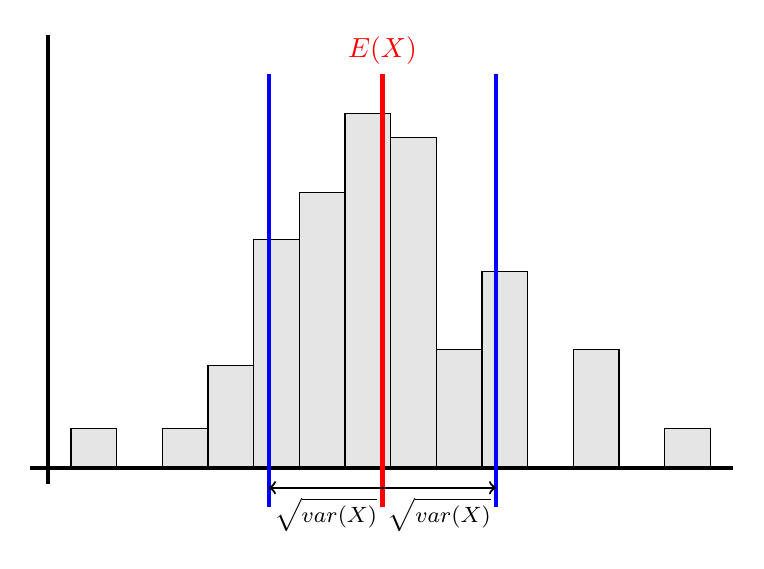
\begin{tikzpicture}[xscale=0.58, yscale=1]
	\def\values{{0.5, 0, 0.5, 1.3, 2.9, 3.5, 4.5, 4.2, 1.5, 2.5, 0, 1.5, 0, 0.5}}
	\def\EWert{7.32}
	\def\StAbw{2.49}
	
	%Histogramm werte
	\foreach \i in {0,1,...,13}
		\filldraw[draw=black, fill=gray!20] (\i+0.5, 0) rectangle (\i+1.5, \values[\i]);
	
	%Achsen
	\draw[ultra thick] (0,-0.2) -- (0,5.5);
	\draw[ultra thick] (-0.4, 0) -- (15,0);
	
	%Erwartungswert
	\draw[ultra thick, red] (\EWert,-0.5) -- (\EWert,5);
	\node[above, red] at (\EWert,5){$E(X)$};
	
	%Varianz
	\draw[ultra thick, blue] (\EWert-\StAbw,-0.5) -- (\EWert-\StAbw,5);
	\draw[ultra thick, blue] (\EWert+\StAbw,-0.5) -- (\EWert+\StAbw,5);
	\draw [<->, thick] (\EWert-\StAbw, -0.25) -- (\EWert+\StAbw, -0.25);
	\node[below] at ({\EWert-(\StAbw/2)},-0.25){\footnotesize$\sqrt{var(X)}$};
	\node[below] at ({\EWert+(\StAbw/2)},-0.25){\footnotesize$\sqrt{var(X)}$};
	
		
%	\newcommand{\HelpCords}[4]{
%		\draw [help lines] (#1,#2) grid (#3,#4);
%		\foreach \i in {#1,..., #3}
%		\node [below] at (\i,#2) {$\i$};
%		\foreach \i in {#2,..., #4}
%		\node [left] at (#1,\i) {$\i$};
%	}
%	\HelpCords{0}{0}{15}{5.5}
\end{tikzpicture}

\end{minipage}

\hrule

\begin{minipage}{0.42\textwidth}
	\vspace{2mm}
	\subsection{Varianz}
	$\boxed{var(X)=E(X^2)-E(X)^2}= \:E[(X-E(X))^2]$\\[2pt]
	\textbf{Standardabweichung} $\sigma = \sqrt{var(X)}$

	\subsubsection{Kovarianz}
	$cov(X,Y)=E(XY)-E(X)E(Y)=\hspace{-0.8cm}\underbrace{0}_{\text{falls X,Y unabhängig}}$\\[2pt]
	Ist die Kovarianz positiv so tendieren höhere $X$-Werte zu höheren $Y$-Werten.
	\vspace{.2cm}
\end{minipage}
\hspace{0.02\textwidth}
\begin{minipage}{0.56\textwidth}
	\vspace{2mm}
	\subsubsection{Rechenregeln}
		$var(\lambda X)=\lambda^2 var(X) \qquad $ $\lambda, \mu \in \mathbb{R}$\\[4pt]
		$var(X_1+X_2+\ldots+X_n) \neq var(n X)$ \\[4pt]
		$var(X+Y)= 
			\begin{cases}
		  		var(X)+var(Y) & \text{(X,Y unabh.)}\\                
		  		var(X) + var(Y) + 2 \cdot cov(X,Y) & \text{(X,Y abhängig)}\\
			\end{cases} $ \\[4pt]
		$var(X Y)= var(Y)var(X)+var(Y)E(X)^2+var(X)E(Y)^2$ \\
	\vspace{.2cm}
\end{minipage}

\hrule

\subsection{Erwartungswert und Varianz des arithmetischen Mittels}
Es sei eine Folge von unabhängigen Zufallsvariablen $X_1, X_2, \ldots , X_n$ mit gleichem Erwartungswert $ \mu $ und gleicher Varianz $ \sigma^2 $ gegeben. \\
\begin{tabular}{m{0.33\textwidth} m{0.33\textwidth} m{0.33\textwidth}}
	Mittelwert: $M_n=\frac{X_1+\ldots+X_n}{n}$ &
	Erwartungswert: $E(X)=E(M_n) = \mu$  &
	Varianz: $var(M_n)=\frac{1}{n}var(X) = \frac{\sigma ^2}{n} $
\end{tabular}
\vspace{1mm}
\hrule

\subsection{Satz von Tschebyscheff \skript{\pageref{sk-ungleichung-von-tschebyscheff}}}
\begin{tabular}{ll}
  $P(\left| X-E(X) \right|>\varepsilon)\leq\dfrac{var(X)}{\varepsilon^2}$ &
  Wahrscheinlichkeit, dass $X$ um mehr als $\varepsilon$ vom Erwartungswert $E(X)$ abweicht.\\
  $P(|M_{n}-\mu|>\varepsilon)\leq \frac{\sigma^{2}}{\varepsilon^{2}n} $ &
  W'keit, dass $M_{n}$ von $n$ unab. ZV mit Mittelwert $\mu$ und Varianz $\sigma^{2}$ mehr als $\varepsilon$ von $\mu$ abweicht.
\end{tabular}

\begin{minipage}[t]{9cm}
  \subsection{Regression \skript{\pageref{sk-rekursion}}}
  \begin{tabular}{ll}
    Allgemein: & X,Y Zufallsvariable \\
    Gesucht: & Regressionsgerade $y=ax+b$ mit min. Fehler \\
    Fehler: & $E(Y-(aX+b))=0$ \\
  \end{tabular} \\
 
  \textbf{Regressionskoeffizient r} \\
  $r$ ist ein Mass für die Qualität der Regression (standardisiert) \\
  $r^2=\dfrac{cov(X,Y)^2}{var(X)var(Y)}=a^2\cdot\dfrac{var(X)}{var(Y)}$ \\  \\
  Liegt $r$ nahe bei $1$ $\widehat{=}$ gute Approximation\\ \\
 
  \textbf{Mittlerer quadratischer Fehler} \\
  $\Delta^2 = var(Y)(1-r^2) =
  var(Y)\left(1-\dfrac{cov(X,Y)^2}{var(X)var(Y)}\right) $ \\
\end{minipage}
\begin{minipage}[t]{10cm}
  \textbf{Vorgehen:}
  \textcolor{blue}{mit Fehlerberechnung}
	\begin{enumerate}
		\item Tabelle mit bekannten Werten aufstellen:\\
  		\begin{tabular}{|l||l|l||l|l||l|}
  		  \hline
        \textbf{$k$} & \textbf{$x$} & \textbf{$x^2$} & \textbf{$y$} &
  		  \textcolor{blue}{\textbf{$y^2$}} & \textbf{$xy$} \\
  		  \hline \hline
  		  $1$ & $x_1$ & $x_1^2$ & $y_1$ & \textcolor{blue}{$y_1^2$} & $x_1y_1$ \\
  		  \hline
  		  $\vdots$ & $\vdots$ & $\vdots$ & $\vdots$ & \textcolor{blue}{$\vdots$} &
  		  $\vdots$ \\\hline $n$ & $x_n$ & $y_n^2$ & $y_n$ & \textcolor{blue}{$y_n^2$} & $x_ny_n$ \\
  		  \hline
  		  \hline
  		  $\sum$ & $\sum x_k$ & $\sum x_k^2$ & $\sum y_k$ & \textcolor{blue}{$\sum
  		  y_k^2$} & $\sum x_ky_k$ \\
  		  \hline $E$ & $\frac{\sum x_k}{n}$ & $\frac{\sum x_k^2}{n}$ & $\frac{\sum
  		  y_k}{n}$ & \textcolor{blue}{$\frac{\sum y_k^2}{n}$} & $\frac{\sum x_ky_k}{n}$ \\
  		  \hline
  		\end{tabular} 
		\item Varianzen, Kovarianz berechnen: \\
		  $var(X) = E(X^2) - E^2(X)$ \\
		  \textcolor{blue}{$var(Y) = E(Y^2) - E^2(Y)$} \\
		  $cov(X,Y) = E(XY) - E(X)E(Y)$
		\item Koeffizienten \textcolor{blue}{und Fehler} der Gerade berechnen: \\
		  $a=\dfrac{cov(X,Y)}{var(X)}$
		  \textcolor{blue}{$\qquad\Delta^2=var(Y)\left(1-\dfrac{cov(X,Y)^2}
		  {var(X)var(Y)}\right) $} \\
		  $b=E(Y)-aE(X)$
		\item Gerade: \\
		$y=ax+b$
	\end{enumerate}
\end{minipage}

\hrule
